\documentclass[12pt,a4paper]{article}
\usepackage{graphicx,amsmath,amssymb,float,caption,hyperref,fancyhdr}
\usepackage{newtxtext,newtxmath}
\usepackage{geometry,booktabs,tabularx}
\geometry{margin=1in}
\setlength{\headheight}{14.5pt}
\pagestyle{fancy}\fancyhf{}\lhead{IEEE 14-bus: 1 SG + 4 IBR, AGSI++}\rhead{\thepage}
\hypersetup{colorlinks=true,linkcolor=blue,urlcolor=blue}
\title{\textbf{IEEE 14-Bus GFL$\leftrightarrow$GFM Switching with Project AGSI++}\\
\large Full-state implementation and present evidence}
\date{4 August 2026}
\begin{document}
\maketitle

\begin{abstract}
The study uses the configured IEEE 14-bus case, device parameters, and event chronology;
switching remains the project AGSI++. The study profile uses a six-state operational EMF6 SG and 12-state
GFL/GFM switching supersets. A compressed ideal-SG reclose gate converges and returns all
four IBRs to GFL. The 160-s chronology remains fail-closed at 36.040~s because the paper
does not publish the DC-source, post-trip active-power dispatch, or multi-GFM coordination
laws needed to reproduce its islanded trajectory. No values or plots are altered to force recovery.
\end{abstract}

\section{Case, index, and switching}
The 100-MVA, 60-Hz IEEE 14-bus case has one SG at bus 1 and IBRs at buses 2, 3, 6, and 8.
The configured apparent-power dispatch is mapped to $P/Q$ with a documented common angle
(\texttt{PROJECT\_DERIVED}); all device values are read from the source table.
The project index is
\[
J_V=\frac{|V-V_{ref}|}{0.10},\quad J_f=\frac{|f-60|}{0.50},\quad
J_R=\frac{|\mathrm df/\mathrm dt|}{1.0},\quad J_P=\frac{|P_{ref}-P|}{0.20},
\]
\[
J_{SCR}=\max(0,3/SCR-1),\quad J_{lock}=\frac{|v_q|}{0.10},\quad
J_{GRA}=1-GRA,\qquad \mathrm{AGSI}^{++}=\frac{1}{7}\sum J_k .
\]
Each IBR has its own timer. It commits GFL$\to$GFM above $\Gamma_{on}=0.65$ for
$T_{d,on}=0.10$~s and GFM$\to$GFL below $\Gamma_{off}=0.35$ with $GRA=1$ for
$T_{d,off}=1.00$~s. In the full run, IBR1--2 switch at 20.130~s and IBR3--4 at
20.150~s; the action is local, not broadcast. Coordinated SG-reference handback is a
separate declared override used only by the reclose gate.

\begin{figure}[H]\centering
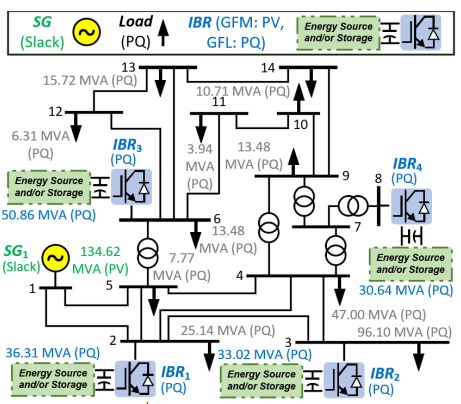
\includegraphics[width=5.90in]{figures/switch_ieee14/ieee14_oneline.png}
\caption{Network and resource locations used by the simulation.}
\end{figure}

\section{Dynamic model}
The SG state is
$x_{SG}=[\delta,\Delta\omega,E'_q,E'_d,E''_q,E''_d]^T$ with the operational
Kundur/EMF6 stator and flux equations. $T_m$ and $E_{fd}$ are equilibrium controls held
constant; governor, AVR, synchronizer, and breaker transients are not claimed.

The GFL superset contains filter current, DC-link, PLL, $P/Q$ PI, current PI, and command-delay
states. GFM contains filter current, DC-link, virtual angle/speed/EMF, voltage PI, current PI,
and delay states. Source values include $L_f=0.15$, $R_f=0.015$, $C_{dc}=0.10$,
$I_{max}=1.2$, $T_d=0.02$, $k_{p,Idq}=0.30$, and $k_{i,Idq}=4.00$.
The paper does not publish the energy-source $I_{dc}$ law, so the implementation closes that
port with ideal instantaneous power balance; this preserves $V_{dc}$ but cannot establish
long-duration energy headroom.

\section{Power-flow operating point}
\begin{table}[H]\centering\caption{Bus power-flow results (pu)}
\resizebox{\textwidth}{!}{% Generated by scripts/reporting/generate_ieee14_switch_report_figures.m.
\begin{tabular}{rrrrrrrr}\toprule
Bus & Type & $|V|$ & $\theta$ (deg) & $P_g$ & $Q_g$ & $P_L$ & $Q_L$ \\ \midrule
1 & REF & 1.06000 & +0.0000 & +2.32393 & -0.16549 & 0.00000 & 0.00000 \\ 
2 & PV & 1.04500 & -4.9826 & +0.40000 & +0.43557 & 0.21700 & 0.12700 \\ 
3 & PV & 1.01000 & -12.7251 & +0.00000 & +0.25075 & 0.94200 & 0.19000 \\ 
4 & PQ & 1.01767 & -10.3129 & +0.00000 & +0.00000 & 0.47800 & -0.03900 \\ 
5 & PQ & 1.01951 & -8.7739 & +0.00000 & +0.00000 & 0.07600 & 0.01600 \\ 
6 & PV & 1.07000 & -14.2209 & -0.00000 & +0.12731 & 0.11200 & 0.07500 \\ 
7 & PQ & 1.06152 & -13.3596 & +0.00000 & +0.00000 & 0.00000 & 0.00000 \\ 
8 & PV & 1.09000 & -13.3596 & +0.00000 & +0.17623 & 0.00000 & 0.00000 \\ 
9 & PQ & 1.05593 & -14.9385 & +0.00000 & +0.00000 & 0.29500 & 0.16600 \\ 
10 & PQ & 1.05098 & -15.0973 & +0.00000 & +0.00000 & 0.09000 & 0.05800 \\ 
11 & PQ & 1.05691 & -14.7906 & +0.00000 & +0.00000 & 0.03500 & 0.01800 \\ 
12 & PQ & 1.05519 & -15.0756 & +0.00000 & +0.00000 & 0.06100 & 0.01600 \\ 
13 & PQ & 1.05038 & -15.1563 & +0.00000 & +0.00000 & 0.13500 & 0.05800 \\ 
14 & PQ & 1.03553 & -16.0336 & +0.00000 & +0.00000 & 0.14900 & 0.05000 \\ 
\bottomrule\end{tabular}
}
\end{table}
\begin{table}[H]\centering\caption{From-end line flows and losses (pu)}
\resizebox{\textwidth}{!}{% Generated by scripts/reporting/generate_ieee14_switch_report_figures.m.
\begin{tabular}{r@{\hspace{0.8em}}r@{\hspace{0.8em}}r@{\hspace{0.8em}}r@{\hspace{0.8em}}r@{\hspace{0.8em}}r@{\hspace{0.8em}}r}\toprule
Line & From & To & $P_{from}$ & $Q_{from}$ & $P_{loss}$ & $Q_{loss}$ \\ \midrule
1 & 1 & 2 & +0.900928 & -0.203057 & +0.014518 & -0.014696 \\
2 & 1 & 5 & +0.418019 & -0.066451 & +0.008475 & -0.019813 \\
3 & 2 & 3 & +0.464318 & -0.000621 & +0.009133 & -0.009246 \\
4 & 2 & 4 & +0.314334 & -0.079982 & +0.005358 & -0.021354 \\
5 & 2 & 5 & +0.209348 & -0.060569 & +0.002332 & -0.031219 \\
6 & 3 & 4 & -0.197092 & -0.022968 & +0.002456 & -0.007604 \\
7 & 4 & 5 & -0.447907 & +0.102332 & +0.002561 & +0.008079 \\
8 & 4 & 7 & +0.017005 & -0.115901 & +0.000000 & +0.002495 \\
9 & 4 & 9 & +0.062330 & -0.021423 & +0.000000 & +0.002062 \\
10 & 5 & 6 & +0.090091 & +0.002266 & -0.000000 & +0.001610 \\
11 & 6 & 11 & +0.130988 & +0.058687 & +0.001540 & +0.003226 \\
12 & 6 & 12 & +0.085939 & +0.026725 & +0.000784 & +0.001631 \\
13 & 6 & 13 & +0.207419 & +0.084233 & +0.002610 & +0.005140 \\
14 & 7 & 8 & -0.268840 & -0.133746 & +0.000000 & +0.013242 \\
15 & 7 & 9 & +0.285846 & +0.015351 & +0.000000 & +0.007516 \\
16 & 9 & 10 & -0.003741 & +0.022196 & +0.000013 & +0.000036 \\
17 & 9 & 14 & +0.056917 & +0.023544 & +0.000403 & +0.000857 \\
18 & 10 & 11 & -0.093754 & -0.035839 & +0.000693 & +0.001622 \\
19 & 12 & 13 & +0.024155 & +0.009094 & +0.000119 & +0.000108 \\
20 & 13 & 14 & +0.093845 & +0.030080 & +0.001359 & +0.002767 \\
\bottomrule\end{tabular}
}
\end{table}

\section{Mode and recovery evidence}
\begin{table}[H]\centering
\begin{tabularx}{\textwidth}{@{}>{\raggedright\arraybackslash}p{0.20\textwidth}X p{0.25\textwidth}@{}}
\toprule Time & Event/index/timer & Committed mode \\ \midrule
20.000--20.130~s & SG trip; local on-timers run & IBR1--2 become GFM \\
20.150~s & remaining local timers mature & IBR3--4 become GFM \\
36.040~s & full chronology exits the validity domain & fail-closed before later events \\
1.000--1.140~s (gate) & compressed SG trip and local timers & all GFL$\to$GFM \\
3.000~s (gate) & ideal SG reference and coordinated handback & all GFM$\to$GFL \\
4.000~s (gate) & Newton converged; $\min|V|=1.033013$ pu & all remain GFL \\
\bottomrule
\end{tabularx}
\end{table}

\begin{figure}[H]\centering
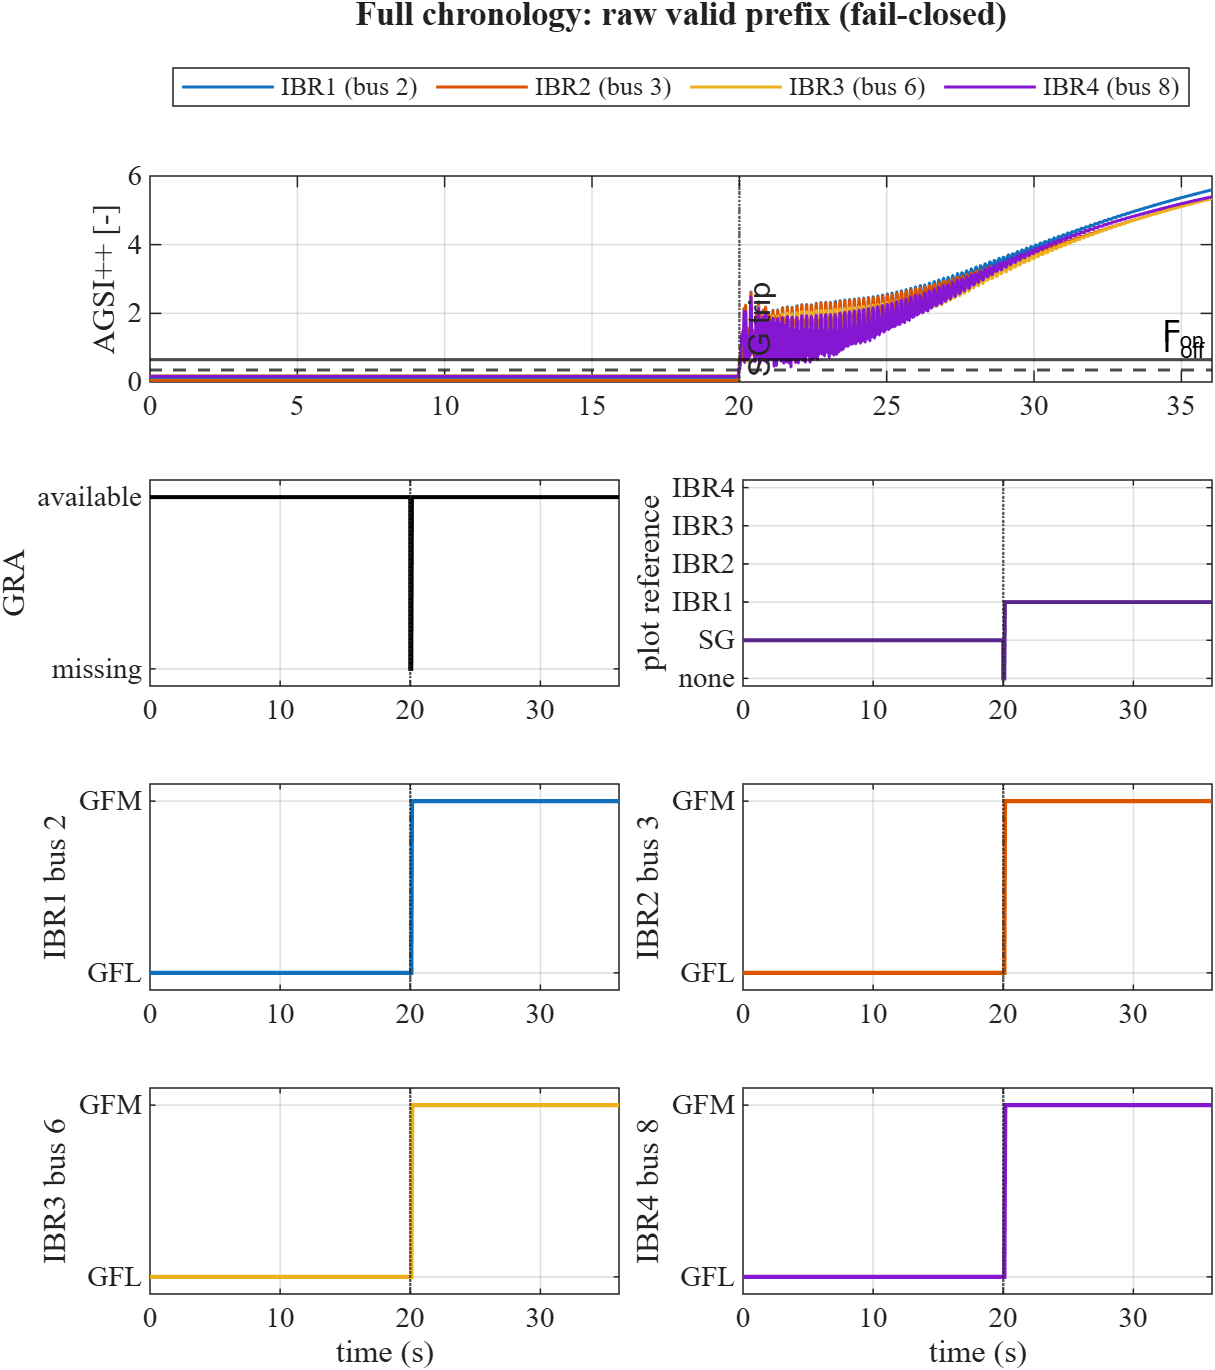
\includegraphics[width=5.90in]{figures/switch_ieee14/padiyar_switch_supervisor.png}
\caption{Full-run AGSI++, GRA, reference, and separate 0=GFL/1=GFM timelines.}
\end{figure}
\begin{figure}[H]\centering
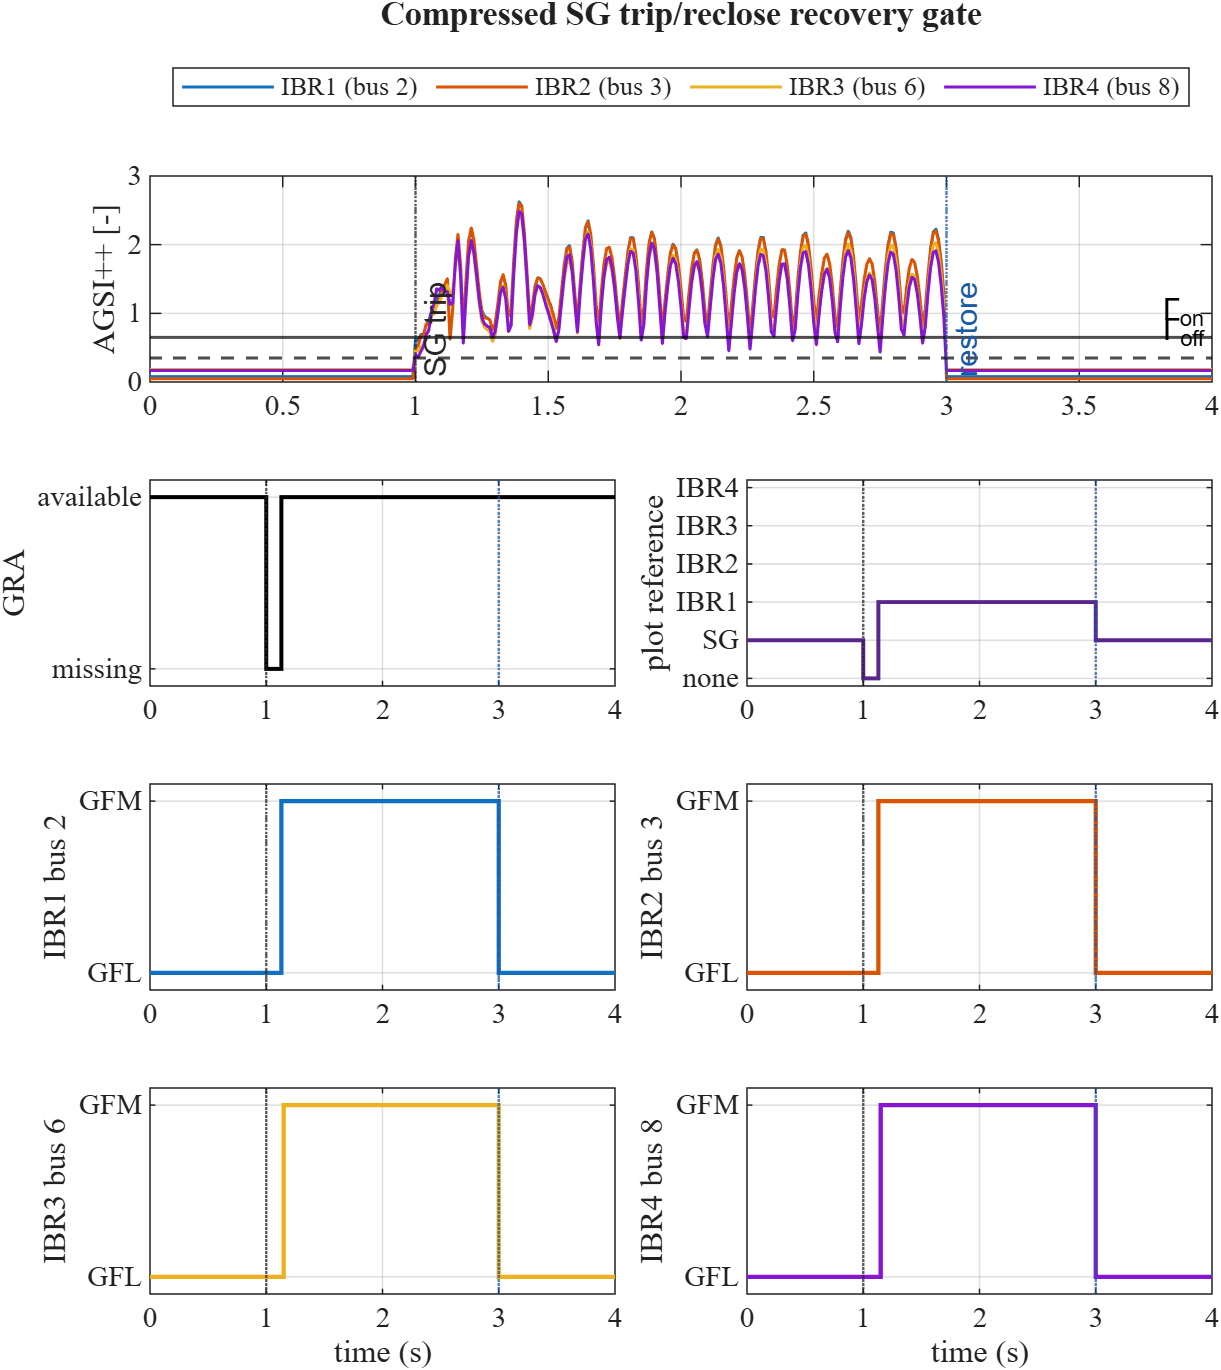
\includegraphics[width=5.90in]{figures/switch_ieee14/padiyar_switch_recovery_supervisor.png}
\caption{Compressed recovery gate: local switch-up and coordinated SG handback.}
\end{figure}
\begin{figure}[H]\centering
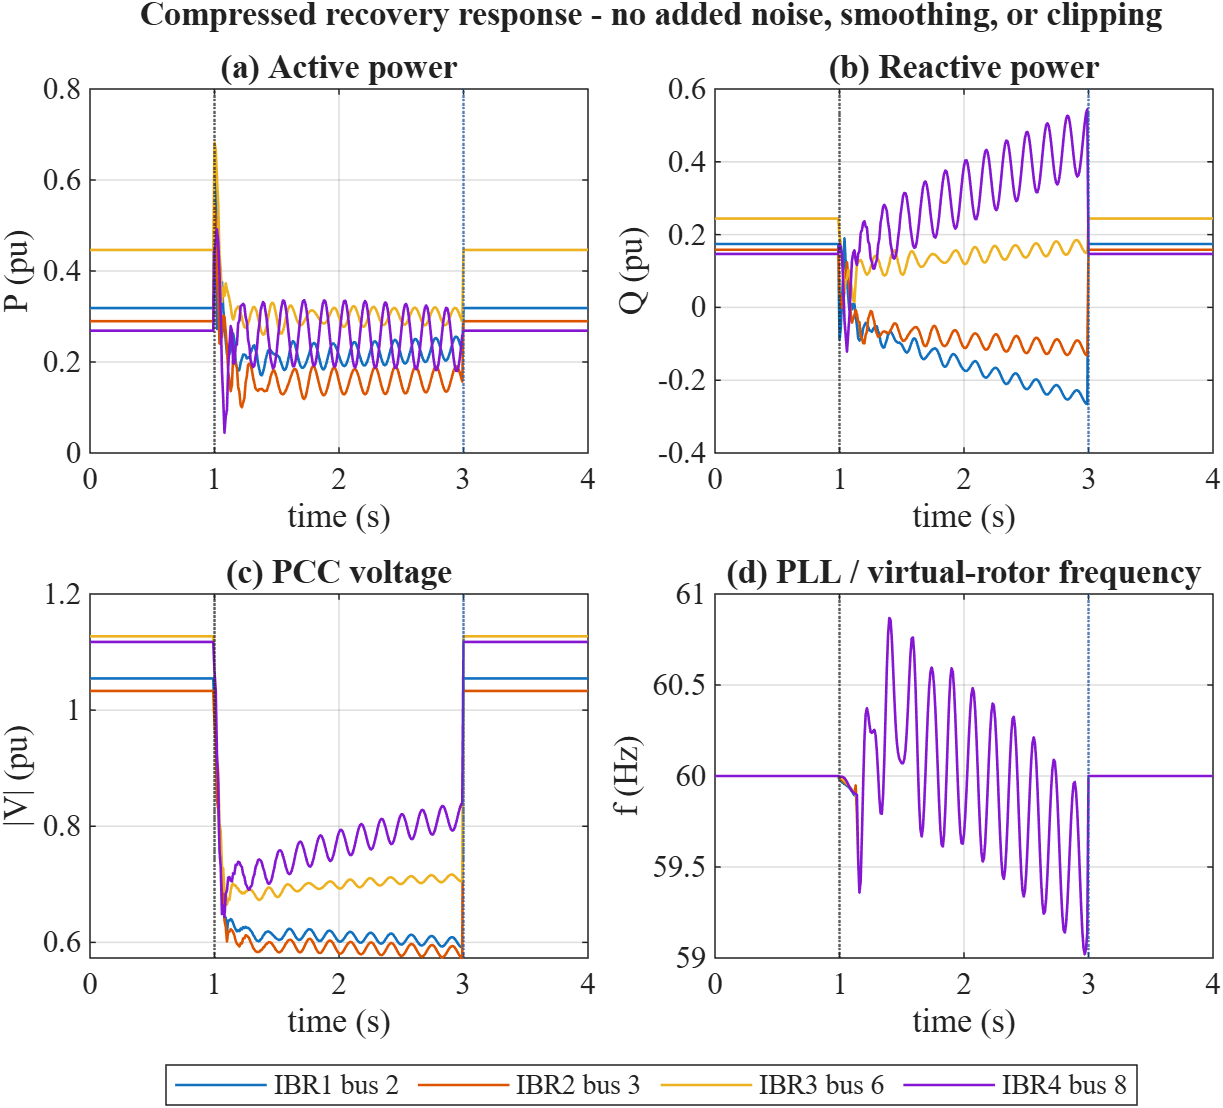
\includegraphics[width=5.90in]{figures/switch_ieee14/padiyar_switch_recovery_response.png}
\caption{Raw recovery-gate $P,Q,|V|,f$ traces; no noise, smoothing, or clipping.}
\end{figure}

Existing tests separately cover no-event, light/severe faults, load steps, SG trip, and SG
reclose. The long full-state run currently reaches only the SG-trip portion; it does not validate
the scheduled 50-s load step, 85-s fault, 110-s line trip, or 145-s restoration. The remaining
gap is a missing dispatch/energy/reference-coordination contract, not merely SG state order.

\section{Reproduction}
\begin{verbatim}
pf_init_paths;
addpath(fullfile('scripts','reporting'));
generate_ieee14_switch_report_figures;
\end{verbatim}
The generator and all solvers are project-owned MATLAB. SSSA and fault-map sections are omitted
to keep the report focused on IBR switching.
\end{document}
